% figures/detect/fig_anomalies.tex — loads PDF exported from NB04
% Requires \usepackage{graphicx}. Export the anomaly scatter / timeline
% as figures/detect/anomalies.pdf.
\begin{figure}[!ht]
    \centering
    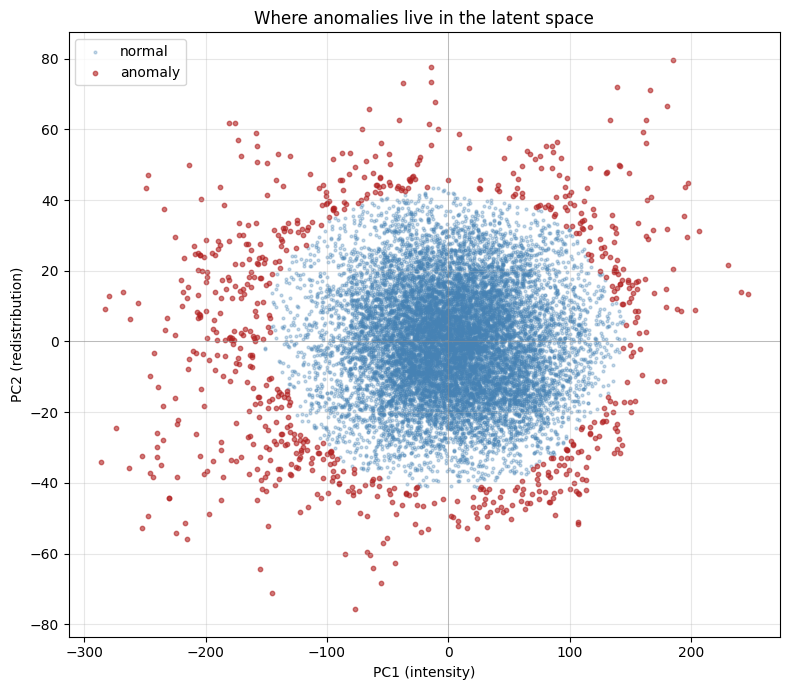
\includegraphics[width=0.9\textwidth]{figures/data_pipeline/anomalies.png}
    \caption[Isolation Forest anomalies across the record.]{\textbf{Discrete
    anomalous events, spread across the record.} The Isolation Forest flags
    \SI{5}{\percent} of days (730) as anomalous in the PC1--PC2 plane. They cluster
    in 2009--2010 (158 days), 2012--2013 (100) and 2018 (66), with no trend over
    time --- corroborating the early-warning null from a different method. These
    moments become perceptible texture (grammar principle~P3) in
    Chapter~\ref{ch:translate}.}
    \label{fig:anomalies}
\end{figure}
